\subsection{x,y,z,SNR Filter}
The point cloud's points are passed through a first static filtering stage to remove points caused by noise, clutter or targets outside of the area of interest before being used for further processing.
This static filtering stage consists of four different filters, filtering out points by different attributes:
\begin{enumerate}
    \item Filtering by $SNR$: All points with a $SNR$ lower than \SI{12}{\deci\bel} are filtered out to remove points with a low signal and those that might be caused by noise or clutter.
    \item Filtering by $z$ coordinate: All points below a $z$ value of \SI{0}{\meter} and above \SI{2}{\meter} are filtered out to remove points caused by the ground or the ceiling.
    \item Filtering by $y$ coordinate: All points below a $y$ value of \SI{0.3}{\meter} are filtered out to remove points created by the driver's feet.
    \item Filtering by $\phi$: All points with an azimuth bigger than \SI{85}{\degree} are filtered out to remove points that are outside the area of interest.
\end{enumerate}
\textit{Note: The origin of the points' coordinate system is the sensor itself, so a coordinate of $(\SI{0}{\meter},\SI{0}{\meter},\SI{0}{\meter})$ is essentially at the sensor's mounting position and therefore approx. \SI{0.3}{\meter} above the ground.}
\par
As the static filtering stage only keeps points which are relevant in terms of there spatial position and $SNR$ for the following stages, it effectively decreases the computation time of each frame and prevents the following stages from processing invalid data.
The filtered point cloud is then passed to the next stages, the self-speed estimator and the dynamic filtering stage.

\begin{figure}[!htbp]
\centering
\begin{subfigure}{0.24\textwidth}
  \centering
  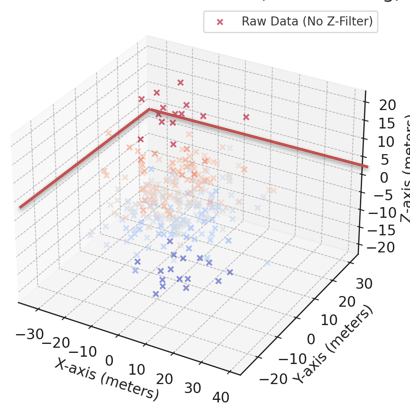
\includegraphics[width=\textwidth]{images/No_filter.png}
  \caption{Input}
\end{subfigure}
\begin{subfigure}{0.24\textwidth}
  \centering
  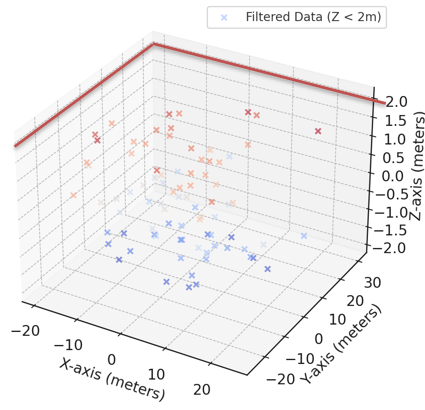
\includegraphics[width=\textwidth]{images/filter.png}
  \caption{Output}
\end{subfigure}
\caption{Example visualization of the input and output when filtering by the value of the $z$ coordinate.}
\label{fig:static_filter_z_example}
\end{figure}
\FloatBarrier\noindent



\subsubsection{Static vs Non-static objects}
In the detected data there will always be static or moving objects in the field of view, this is more prominent when the sensor is mounted in a moving frame.
In this case every thing is moving from the perspective of the sensor, so how does the differentiation happens to identify statis vs non-static objects, this is simple, by leveraging on the doppler effect concept.
Using the doppler effect and understanding it is crutial for this step, as it is what will allow the algorithm to focuse the processing only in the static targets that are detected.

In this case, making the assumption that the sensor is mounted in a vehicle that goes 2 meters per second. With this in consideration, the assumption that all static targets should have a radial speed similar to the 2 meters per second.
This speed cannot be the same as the angle of detection can affect, the accuracy that may be obtained through the chirp configuration, etc.
Multiple variables can be added into this "equation", but the assumption that the static targets measured radial speed is close to the vehicle speed we can know which target to keep and which target to discard with only this paramter.

However that leaves us with the problem of how to group such targets. At this point the RANSAC algorithm becomes useful, as it will do the grouping for us, by ussing the radial speed.
